\documentclass{article}

% if you need to pass options to natbib, use, e.g.:
%     \PassOptionsToPackage{numbers, compress}{natbib}
% before loading neurips_2020

% ready for submission
\usepackage[final]{neurips_2020}

% to compile a preprint version, e.g., for submission to arXiv, add add the
% [preprint] option:
%     \usepackage[preprint]{neurips_2020}

% to compile a camera-ready version, add the [final] option, e.g.:
%     \usepackage[final]{neurips_2020}

% to avoid loading the natbib package, add option nonatbib:
%\usepackage[nonatbib]{neurips_2020}

\usepackage[utf8]{inputenc} % allow utf-8 input
\usepackage[T1]{fontenc}    % use 8-bit T1 fonts
\usepackage{hyperref}       % hyperlinks
\usepackage{url}            % simple URL typesetting
\usepackage{booktabs}       % professional-quality tables
\usepackage{amsfonts}       % blackboard math symbols
\usepackage{nicefrac}       % compact symbols for 1/2, etc.
\usepackage{microtype}      % microtypography

\usepackage{graphicx}
\graphicspath{ {./figs/} }

\title{Randomized Overdrive Neural Networks}

% The \author macro works with any number of authors. There are two commands
% used to separate the names and addresses of multiple authors: \And and \AND.
%
% Using \And between authors leaves it to LaTeX to determine where to break the
% lines. Using \AND forces a line break at that point. So, if LaTeX puts 3 of 4
% authors names on the first line, and the last on the second line, try using
% \AND instead of \And before the third author name.

\author{%
  Christian J. ~Steinmetz \\
  Queen Mary University of London\\
  \texttt{c.j.steinmetz@qmul.ac.uk} \\
  \And
  Joshua D.~Reiss \\
  Queen Mary University of London \\
  \texttt{joshua.reiss@qmul.ac.uk} \\
}

\begin{document}

\maketitle

\begin{abstract}
By processing audio signals in the time-domain with randomly weighted temporal convolutional networks (TCNs),
we uncover a wide range of novel, yet controllable overdrive effects.
We discover that architectural aspects, such as the depth of the network, 
the kernel size, the number of channels, the activation function, as well as the weight initialization, 
all have a clear impact on the sonic character of the resultant effect, without the need for training. 
In practice, these effects range from conventional overdrive and distortion,
to more extreme effects, as the receptive field grows, similar to a fusion of distortion, equalization, delay, and reverb.  
To enable use by musicians and producers, we provide a real-time plugin implementation.
This allows users to dynamically design networks, listening to the results in real-time.
We provide a demo, along with code and builds at \url{https://ronn.ml}.
\end{abstract} 


% The TCN architecture can be viewed as a nonlinear waveshaper with memory
% equal to receptive field of the causal convolutional network. 

\section{Introduction}

Throughout the history of audio technology, engineers, circuit designers, 
and particularly guitarists, have searched for novel sonic effects as a result of clipping or distorting audio signals. 
These distortion effects were first discovered by pushing early guitar amplifiers beyond their operating range, 
or, in some cases, from the accidental damage to amplifiers or speakers \cite{shepherd2003distortion}. 
These pursuits are a clear example of creators taking advantage of the limitations of their tools for creative effect.
Distortion has permeated genres such as blues, jazz, rock, and metal, and also play a central role in modern pop and hip-hop styles.
Whether it be vacuum tubes, diodes, transistors, integrated circuits, or software-based digital models,
it may appear as if nearly all the methods of generating distortion-based effects have been exhausted.
We claim this may not be the case, as we will examine the potential of neural networks to generate a new class of distortion-based effects. 

Neural networks are far from new, and in fact they arose in the same era that blues guitarists began their experiments with distortion \cite{schmidhuber2015deep}.
Yet, only more recently, following the emergence of modern deep learning approaches, 
have neural networks become feasible for audio signal processing tasks \cite{purwins2019deep}.
Interestingly, these methods have shown to be successful in emulating the characteristics of amplifiers and distortion effects 
\cite{schmitz2018nonlinear, zhang2018lstm, damskagg2019distortion, martinez2019nonlinear}.
While these approaches have largely been successful in this emulation task, the aim of our work deviates from these virtual effect modeling approaches.
In a similar spirit to the guitarists using their amplifiers in a fashion unintended by the original designer,
we propose the apparent abuse of neural networks by utilizing randomly initialized networks as complex signal processing devices
to distort, transform, and warp audio signals for creative effect. 

\section{Method}
\subsection{Architecture}

We select a convolutional architecture as it provides a parameter efficient method for processing arbitrary length sequences, 
and from the perspective of audio signal processing, it can be considered a series of filters and nonlinear waveshapers.
The temporal convolutional network (TCN) formalizes the application of convolutional models operating on 1-dimensional sequences,
and outlines a set of design choices ideal for various sequence modeling tasks \cite{bai2018tcn}. 
Causal convolutions are a core component of this formulation, in which outputs are predicted considering only past values,
so information from the future does not "leak" into current predictions. 
Additionally, these networks are generally built to be fully convolutional, 
so they can process input signals of arbitrary length, and will produce an output signal with length proportional to the input length \cite{long2015fcn}.

With standard causal convolutions the receptive field grows linearly as the depth of the network increases. 
This makes it challenging to achieve models that are able to consider larger time contexts. 
To address this, the TCN incorporates dilated convolutions, which inserts zeros within the taps of the convolutional kernels, 
effectively increasing the size of the kernel without additional computation \cite{oord2016wavenet}. 
To increase the receptive field more rapidly, an exponentially increasing dilation factor is generally applied at each layer in the network. 
In addition, residual connections are used at each layer to further stabilize gradient flow, 
but since we do not aim to train these networks we omit them \cite{he2016deep}.
The overall TCN architecture in our implementation can then be viewed as a simple connection of blocks containing
only 1-dimensional convolutions followed by a nonlinear activation. 

\subsection{Implementation}
For the real-time implementation, \texttt{ronn}, we utilize the JUCE framework\footnote{\url{https://github.com/juce-framework/JUCE}},
which enables us to create a VST/AU plugin for use in popular digital audio workstations (DAWs).
In order to construct the TCN models, we utilize PyTorch \cite{pytorch}, which features a C++ API. 
This enabled us to develop our own parameterized neural network module class that can be instantiated within the main JUCE plugin.
By connecting this class with the user interface, the on-screen controls, as shown in Figure \ref{fig:ui},
can be used to dynamically construct new networks, all in a paradigm that allows for real-time interaction. 

A challenge arises since these models are fully convolutional,
yet the plugin requires that all processing occur on a block-by-block basis. 
Additionally, we utilize convolutions without padding, so the output is often smaller than the input. 
To address this, we construct a look-back buffer large enough so the output sequence matches the length of the input block. 
This buffer stores a sufficient number of past input samples, along with the samples from the current block, as demonstrated in Figure \ref{fig:diagram}. 
In practice, we found this approach produces no perceivable discontinuities at the frame boundaries. 
As expected, as the size of the receptive field increases ($\geq$ 2 seconds), the computational load increases, 
causing the plugin to perform in less than real-time.

To address the significant computational overhead imposed by deeper models, 
we introduce the ability to swap traditional convolutions with depthwise convolutions \cite{howard2017mobilenets}.
These convolutions greatly reduce the computational overhead by convolving $K$ filters with only a single input channel each. 
With this approach we were able to run models with larger receptive fields in real-time on the CPU,
making a wider range of effects achievable on general purpose hardware utilized by musicians and producers. 

We also take advantage of the reality that the TCN can produce any number of output channels, 
which allows us to generate a stereo output signal, given only a monophonic input signal. 
In our listening, we found that this often produced interesting spatialized results. 
This configuration also supports stereo inputs, which can result in interesting cross-channel behavior. 
Finally, there is a global seed control so that every random state can be recovered, enabling users to return to previous effects.

\section{Discussion}

We propose the use of randomly weighted TCNs as complex, time-domain audio signal processing devices. 
We find that adjusting various architectural aspects results in the ability to generate a wide range of compelling sonic effects.
Additionally, there appears to be a clear link between different aspects of the architecture and the characteristics of the generated effect, 
which enables a level of interpretable control. 
While deep networks pose a challenge for real-time implementation due to significant compute overhead, 
we are able to provide a real-time implementation with some careful design choices. 
This plugin enables the use of this set of effects within popular DAWs. 
With a simplified interface, musicians and producers without machine learning experience can easily take advantage of these effects.
While we have only investigated feedforward architectures, 
it reasons that we could achieve a wider range of effects with the addition of recurrent pathways in the networks.

\section*{Broader Impact}
In this work we apply existing neural network approaches for processing audio signals in a creative context.
Since we do not utilize any training data in this process there is a relatively low risk of bias arising here. 
Potential biases in the processing of signals may arise from the randomized network weights,
although such biases are not chosen intentionally, and reflect the underlying characteristics of these generated effects,
representing only a limited set of audio effects afforded by the system.

\bibliography{references}{}
\bibliographystyle{plain}

\newpage
\section*{Supplementary materials}

\begin{figure}[h]
  \centering
  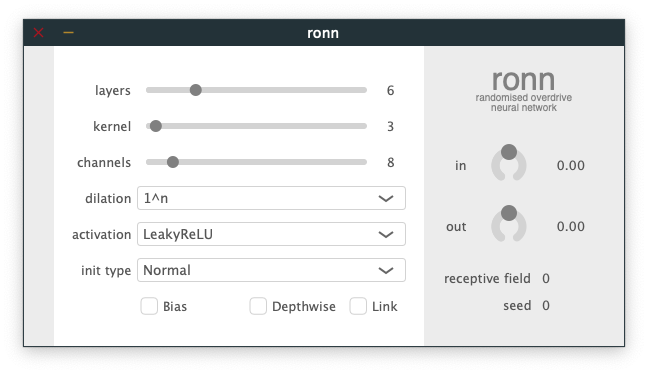
\includegraphics[width=0.9\textwidth]{ronn-vst-ui.png}  
  \caption{Real-time plugin user interface featuring a series of sliders and selection boxes, 
  enabling users to dynamically construct various TCN architectures while listening to the results.
  When the user adjusts any of the on-screen controls, a callback will run, 
  constructing a neural network with the new architectural design. 
  On the bottom right, indicators show the receptive field of the current model in milliseconds, 
  the number of parameters within the current network, as well as the global seed. 
  %The function of each of the user interface controls are as follows: \\ \\
  %\texttt{layers} the number convolutional blocks, or depth of the network. \\
  %\texttt{kernel} the number of taps in all convolutional filters.\\
  %\texttt{channels} the number of convolutional output channels in each block.\\
  %\texttt{dilation} the dilation growth factor, where the dilation is a function of the layer index $n$.\\
  %\texttt{activation} the nonlinear activation function applied at the end of each convolutional block.\\
  %\texttt{init type} the weight initialization mechanism used for the convolutional kernels.\\
  %The \texttt{in} and \texttt{out} sliders adjust the input and output gain, which will act a drive control.
  }
  \label{fig:ui}
\end{figure}

\begin{figure}
  \centering
  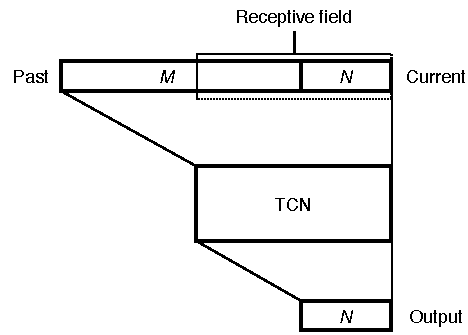
\includegraphics[width=0.55\textwidth]{plugin-diagram.pdf}  
  \caption{Block diagram outlining the block-based processing utilized in the plugin. 
  The look-back buffer is shown at the top, which consists of $N$ samples from the current input block, 
  concatenated with $M$ past input samples. The number of stored past samples $M$ is a function 
  of the receptive field of the TCN, shown in the dotted box, and the block size. 
  $M$ is selected such that the entire buffer of size $M+N$ will produce an output of $N$ samples.
  Recall that since padding is not used, the output of each convolutional block will be smaller than the input. 
  When the receptive field is quite large, producing the output block (e.g. $\approx 10$ ms)
   may require processing multiple seconds of audio.}
  \label{fig:diagram}
\end{figure} 

%\begin{table*}[h]
%  \centering
%   \begin{tabular} {c}
%    \toprule
%    
%    \end{tabular} 
%    \caption{}
%    \label{tab:}   
%\end{table*}

\end{document}
